%%%%%%%%%%%%%%%%%%%%%%%%%%%%%%%%%%%%%%%%%%%%%%%%%%%%%%%%%%%%
%%  NE 155
%%

\documentclass[xcolor=x11names,compress, handout]{beamer}

\definecolor{CoolBlack}{rgb}{0.0, 0.18, 0.39}
%% General document %%%%%%%%%%%%%%%%%%%%%%%%%%%%%%%%%%
\usepackage{graphicx}
\usepackage{tikz}
\usetikzlibrary{decorations.fractals}
\usepackage{hyperref}
%%%%%%%%%%%%%%%%%%%%%%%%%%%%%%%%%%%%%%%%%%%%%%%%%%%%%%

%% Beamer Layout %%%%%%%%%%%%%%%%%%%%%%%%%%%%%%%%%%
\useoutertheme[subsection=false,shadow]{miniframes}
\useinnertheme{default}
\usefonttheme{serif}
\usepackage{palatino}
\usepackage{tabu}
% Links
\usepackage{hyperref}
\definecolor{links}{HTML}{003262}
\hypersetup{colorlinks,linkcolor=,urlcolor=links}

% addition of color
\usepackage{xcolor}
\definecolor{CoolBlack}{rgb}{0.0, 0.18, 0.39}
\definecolor{byellow}{rgb}{0.55037, 0.38821, 0.06142}
\definecolor{dgreen}{rgb}{0.,0.6,0.}
\definecolor{RawSienna}{cmyk}{0,0.72,1,0.45}
\definecolor{forestgreen(web)}{rgb}{0.13, 0.55, 0.13}
\definecolor{cardinal}{rgb}{0.77, 0.12, 0.23}

\setbeamerfont{title like}{shape=\scshape}
\setbeamerfont{frametitle}{shape=\scshape}

\setbeamercolor*{lower separation line head}{bg=CoolBlack}
\setbeamercolor*{normal text}{fg=black,bg=white}
\setbeamercolor*{alerted text}{fg=dgreen} % just testing; I think this looks better
\setbeamercolor*{example text}{fg=black}
\setbeamercolor*{structure}{fg=black}

\setbeamercolor*{palette tertiary}{fg=black,bg=black!10}
\setbeamercolor*{palette quaternary}{fg=black,bg=black!10}

% Margins
\usepackage{changepage}

\mode<presentation>
{
  \definecolor{berkeleyblue}{HTML}{003262}
  \definecolor{berkeleygold}{HTML}{FDB515}
  \usetheme{Boadilla}      % or try Darmstadt, Madrid, Warsaw, Boadilla...
  %\usecolortheme{dove} % or try albatross, beaver, crane, ...
  \setbeamercolor{structure}{fg=berkeleyblue,bg=berkeleygold}
  \setbeamercolor{palette primary}{bg=berkeleyblue,fg=white} % changed this
  \setbeamercolor{palette secondary}{fg=berkeleyblue,bg=berkeleygold} % changed this
  \setbeamercolor{palette tertiary}{bg=berkeleyblue,fg=white} % changed this
  \usefonttheme{structurebold}  % or try serif, structurebold, ...
  \useinnertheme{circles}
  \setbeamertemplate{navigation symbols}{}
  \setbeamertemplate{caption}[numbered]
  \usebackgroundtemplate{}
}
%---

\renewcommand{\(}{\begin{columns}}
\renewcommand{\)}{\end{columns}}
\newcommand{\<}[1]{\begin{column}{#1}}
\renewcommand{\>}{\end{column}}

% adding slide numbers
\addtobeamertemplate{navigation symbols}{}{%
    \usebeamerfont{footline}%
    \usebeamercolor[fg]{footline}%
    \hspace{1em}%
    \insertframenumber/\inserttotalframenumber
}

% equation stuff
\newcommand{\Macro}{\ensuremath{\Sigma}}
\newcommand{\Sn}{\ensuremath{S_N} }
\newcommand{\vOmega}{\ensuremath{\hat{\Omega}}}
\usepackage{mathrsfs}
\usepackage[mathcal]{euscript}
\usepackage{amssymb}
\usepackage{amsthm}
\usepackage{epsfig}
\usepackage{amsmath}
%%%%%%%%%%%%%%%%%%%%%%%%%%%%%%%%%%%%%%%%%%%%%%%%%%
% title stuff for footer
\title{NE 155}
\author{R.\ N.\ Slaybaugh}
\date{April 15, 2021}

\begin{document}

%%%%%%%%%%%%%%%%%%%%%%%%%%%%%%%%%%%%%%%%%%%%%%%%%%%%%%
%%%%%%%%%%%%%%%%%%%%%%%%%%%%%%%%%%%%%%%%%%%%%%%%%%%%%%
\begin{frame}
\title{NE 155\\Introduction to Numerical Simulations in Radiation Transport}
\subtitle{Introduction to Monte Carlo}
\titlepage
\end{frame}

%%%%%%%%%%%%%%%%%%%%%%%%%%%%%%%%%%%%%%%%%%%%%%%%%%%%%%
%%%%%%%%%%%%%%%%%%%%%%%%%%%%%%%%%%%%%%%%%%%%%%%%%%%%%%
\begin{frame}{Learning Objectives}

\begin{columns}
  \begin{column}{0.5\textwidth}
    \begin{enumerate}
    \item Define Monte Carlo simulation
    \item Understand the history of Monte Carlo methods
    \item Justify the choice of Monte Carlo for radiation transport
    \item Understand the mathematical validity of Monte Carlo for radiation transport
    \end{enumerate}
  \end{column}
  \begin{column}{0.5\textwidth}
  	\begin{figure}
  	\begin{center}
  		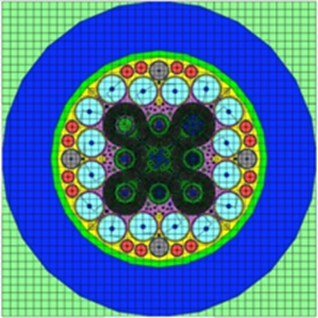
\includegraphics[height=2in,clip]{../figs/atr-model}
  		%http://www.ornl.gov/science-discovery/more-science/mathematics/nuclear-systems-modeling-and-simulation
	\end{center}
  	\end{figure}
  \end{column}
\end{columns}

Notes derived from Jasmina Vujic and Paul Wilson
\end{frame}

%Patterson and Henesey; computer architecture bible; written at berkeley


%%%%%%%%%%%%%%%%%%%%%%%%%%%%%%%%%%%%%%%%%%%%%%%%%%%%%%
%%%%%%%%%%%%%%%%%%%%%%%%%%%%%%%%%%%%%%%%%%%%%%%%%%%%%%
\begin{frame}{What is Monte Carlo?}

  \begin{itemize}
  \item The use of \textit{random processes} to determine a 
        \textit{statistically-expected} solution to a problem
  \vspace*{1em}
  \item Random processes can fulfill two roles:
  \begin{itemize}
    \item Statistical approximation to \alert{mathematical equations}
    \item Statistical approximations to \alert{physical processes}
  \end{itemize}   
 \vspace*{1em} 
  \item Construct a random process for a problem, 
  \item Carry out a numerical simulation by N-fold sampling from a random \# sequence
\end{itemize}
\end{frame}


%%%%%%%%%%%%%%%%%%%%%%%%%%%%%%%%%%%%%%%%%%%%%%%%%%%%%%
%%%%%%%%%%%%%%%%%%%%%%%%%%%%%%%%%%%%%%%%%%%%%%%%%%%%%%
\begin{frame}{Historical Perspective}

  \begin{itemize}
  \item Comte du Buffon (1777): needle tossing experiment to calculate $\pi$
  \pause
  \item Laplace (1786): random points in a rectangle to calculate $\pi$
    \pause
  \item Lord Kelvin (1901): used random sampling to aid in evaluating time integrals associated with kinetic theory of gases
    \pause
  \item Fermi (1930): was among the first to use random sampling methods to study neutron moderation while still in Rome, Italy
    \pause
  %\item Manhattan project (40’s): simulations during the initial development of nuclear weapons. Fermi, von Neumann and Ulam coined the term ``Monte Carlo"
  \item 1947: Fermi, von Neumann, Frankel, Metropolis, Ulam, and others developed computer-oriented Monte Carlo method at Los Alamos to trace neutrons through fissionable materials; coined the term ``Monte Carlo"
    \pause
  \item Berger (1963): first complete coupled electron-photon transport code 
\end{itemize}
\end{frame}


%%%%%%%%%%%%%%%%%%%%%%%%%%%%%%%%%%%%%%%%%%%%%%%%%%%%%%
%%%%%%%%%%%%%%%%%%%%%%%%%%%%%%%%%%%%%%%%%%%%%%%%%%%%%%
\begin{frame}{Evaluate $\pi$ by Random Sampling}

\begin{columns}
  \begin{column}{0.6\textwidth}
    \begin{itemize}
    \item Pierre-Simon Laplace 
    \item Born: 23 March 1749
    \item Died: 5 March 1827 (aged 77)
    \item Nationality and Residence: France
    \item Fields: Astronomy and Mathematics
    \item Institutions: Ecole Militaire; Alma mater: University of Caen
    \end{itemize}
    \vspace*{0.5 em}
    Marquis Pierre-Simon de Laplace, ``Theorie Analytique des Probabilities, Livre 2",  \textit{Ouvres Completes de Laplace}, de L'Academie des Sciences, Paris, \textbf{7}, part 2, 356-366 (1786).
  \end{column}
  \begin{column}{0.4\textwidth}
  	\begin{figure}
  	\begin{center}
  		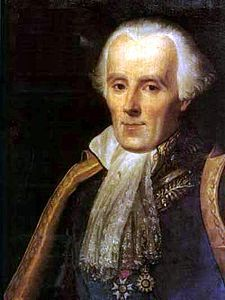
\includegraphics[height=2in,clip]{../figs/laplace}
  		%\caption{Laplace}
	\end{center}
  	\end{figure}
  \end{column}
\end{columns}
\end{frame}


%%%%%%%%%%%%%%%%%%%%%%%%%%%%%%%%%%%%%%%%%%%%%%%%%%%%%%
%%%%%%%%%%%%%%%%%%%%%%%%%%%%%%%%%%%%%%%%%%%%%%%%%%%%%%
\begin{frame}{Evaluate $\pi$ by Random Sampling}

\begin{columns}
  \begin{column}{0.45\textwidth}
  	\begin{figure}
  	\begin{center}
  		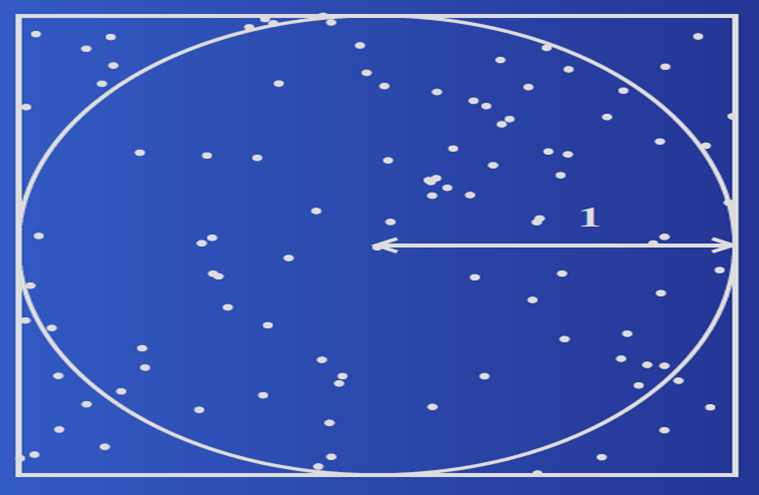
\includegraphics[height=2in,clip]{../figs/pi-circle}
	\end{center}
  	\end{figure}
  \end{column}
  \begin{column}{0.55\textwidth}
    \begin{itemize}
    \item Area of square, $A_s= 4$
    \item Area of circle, $A_c = \pi$
    \item Fraction of random points \\in circle
    \[p = \frac{A_c}{A_s} = \frac{\pi}{4}\]
    \item Random points = $N$
    \item Random points in circle  = $N_c$, $\therefore$
    \[p = \frac{N_c}{N}\:; \quad \pi = \frac{4N_c}{N}\]
    \end{itemize}
  \end{column}
\end{columns}
\end{frame}


%%%%%%%%%%%%%%%%%%%%%%%%%%%%%%%%%%%%%%%%%%%%%%%%%%%%%%
%%%%%%%%%%%%%%%%%%%%%%%%%%%%%%%%%%%%%%%%%%%%%%%%%%%%%%
\begin{frame}{Manhattan Project}

\begin{columns}
  \begin{column}{0.5\textwidth}
    \begin{itemize}
    \item The first human engineered nuclear detonation, 
    the Trinity Test in New Mexico.
    \item Active: 1942--1945
    \item Branch: U.S.\ Army Corps of Engineers
    \item Monte Carlo Pioneers:
    \begin{itemize}
      \item Enrico Fermi,
      \item Stanislaw Ulam,
      \item John von Neumann, 
      \item Robert Richtmeyer, 
      \item Nicholas Metropolis
    \end{itemize}
    \end{itemize}
  \end{column}
  \begin{column}{0.5\textwidth}
  	\begin{figure}
  	\begin{center}
  		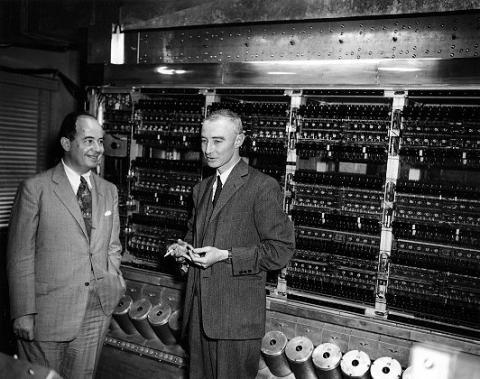
\includegraphics[height=1.75in,clip]{../figs/OppieNeumannMANIAC}
  		\caption{Oppenheimer, von Neumann, MANIAC}
  		%http://www.atomicheritage.org/history/computing-and-manhattan-project
	\end{center}
  	\end{figure}
  \end{column}
\end{columns}
\pause
Nicholas Metropolis, S.\ Ulam. ''The Monte Carlo Method," J\textit{ournal of the American Statistical Association}, \textbf{44}, No.\ 247, 335-341 (Sep. 1949).
\end{frame}


%%%%%%%%%%%%%%%%%%%%%%%%%%%%%%%%%%%%%%%%%%%%%%%%%%%%%%
%%%%%%%%%%%%%%%%%%%%%%%%%%%%%%%%%%%%%%%%%%%%%%%%%%%%%%
\begin{frame}{General Purpose MC Codes}

\begin{itemize}
\item \alert{MCNP}: developed at LANL, distributed via RSICC, \href{http://rsicc.ornl.gov}{http://rsicc.ornl.gov}
%
%\item PENELOPE: developed and maintained at U Barcelona, distributed via the Nuclear Energy Agency (http://www.nea.fr/abs/html/nea-1525.html

\item \alert{Geant4}: developed by a large collaboration in the HEP community, \href{ http://geant4.web.cern.ch/geant4/}{http://geant4.web.cern.ch/geant4/}

\item \alert{EGSnrc}: developed at NRC (Canada), \href{http://www.irs.inms.nrc.ca/EGSnrc/EGSnrc.html}{http://www.irs.inms.nrc.ca/EGSnrc/EGSnrc.html}

\item \alert{SERPENT}: Developed by Dr. Jaakko Leppanen, VTT, Finland, \href{ http://montecarlo.vtt.fi/}{http://montecarlo.vtt.fi/}

\item \alert{Shift}: developed at ORNL, distributed via RSICC, \href{http://rsicc.ornl.gov}{http://rsicc.ornl.gov}

\end{itemize}

\end{frame}


%%%%%%%%%%%%%%%%%%%%%%%%%%%%%%%%%%%%%%%%%%%%%%%%%%%%%%
%%%%%%%%%%%%%%%%%%%%%%%%%%%%%%%%%%%%%%%%%%%%%%%%%%%%%%
\begin{frame}{Evaluate $\pi$ by Random Sampling (math)}

\begin{columns}
  \begin{column}{0.3\textwidth}
  	\begin{figure}
  	\begin{center}
  		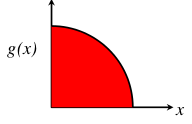
\includegraphics[height=0.75in,clip]{../figs/quarter-circle}
	\end{center}
  	\end{figure}
  \end{column}
  \begin{column}{0.7\textwidth}
    \begin{equation}
      g(x) = \sqrt{1 - x^2}	\qquad G = \int_0^1 g(x)dx = \frac{\pi}{4} \nonumber
    \end{equation}
  \end{column}
\end{columns}
\pause
\begin{equation}
  G = \int_0^1 g(x)dx = (1-0)\overline{g(x)} \nonumber
\end{equation}
Determine $\overline{g(x)}$ by random sampling:\\
\vspace*{0.5em}
\hspace*{2 em}for $k = 1, \dots, N$, choose $\hat{x}_k$ randomly on the interval $(0,1)$,
\[ \overline{g(x)} \equiv \frac{1}{N}\sum_{k=1}^N g(\hat{x}_k) = \frac{1}{N}\sqrt{1 - \hat{x}_k^2}\]

\end{frame}


%%%%%%%%%%%%%%%%%%%%%%%%%%%%%%%%%%%%%%%%%%%%%%%%%%%%%%
%%%%%%%%%%%%%%%%%%%%%%%%%%%%%%%%%%%%%%%%%%%%%%%%%%%%%%
\begin{frame}{Evaluate $\pi$ by Random Sampling (physics)}

\begin{columns}
  \begin{column}{0.3\textwidth}
  	\begin{figure}
  	\begin{center}
  		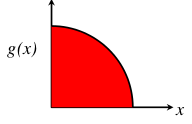
\includegraphics[height=0.75in,clip]{../figs/quarter-circle}
	\end{center}
  	\end{figure}
  \end{column}
  \begin{column}{0.7\textwidth}
    \begin{equation}
      g(x) = \sqrt{1 - x^2}	\qquad G = \int_0^1 g(x)dx = \frac{\pi}{4} \nonumber
    \end{equation}
  \end{column}
\end{columns}
\pause
\vspace*{0.5em}
G = area under curve, \\
\hspace*{0.75 em} = fraction of unit square under curve\\
\vspace*{0.5em}
\hspace*{2 em}for $k = 1, \dots, N$, chose $\hat{x}_k, \hat{y}_k$ randomly on the interval $[0,1]$,\\
\vspace*{0.5em}
$m_N$ = $\#$ of times in $N$ trials that $\hat{x}_k^2 + \hat{y}_k^2 \leq 1$,
\[G = \frac{m_N}{N}\]

\end{frame}


%%%%%%%%%%%%%%%%%%%%%%%%%%%%%%%%%%%%%%%%%%%%%%%%%%%%%%
%%%%%%%%%%%%%%%%%%%%%%%%%%%%%%%%%%%%%%%%%%%%%%%%%%%%%%
\begin{frame}{Why/When Monte Carlo?}

\begin{itemize}
\item Applications that are mathematically equivalent to \textit{integration over many dimensions}
\vspace*{0.25 em}
\begin{itemize}
\item Analytic integration may be impossible
\vspace*{0.25 em}
\item Deterministic numerical integration may be slow and/or require error prone approximations
\end{itemize} 
\vspace*{0.5 em}
\pause
\item However, statistically accurate results can require \textbf{significant computer time}
\item Fortunately, Monte Carlo and parallel computing go well together
\item and we also have Variance Reduction methods
\end{itemize}

\end{frame}


%%%%%%%%%%%%%%%%%%%%%%%%%%%%%%%%%%%%%%%%%%%%%%%%%%%%%%
%%%%%%%%%%%%%%%%%%%%%%%%%%%%%%%%%%%%%%%%%%%%%%%%%%%%%%
\begin{frame}{MC is Used in Many Fields}

\begin{columns}
  \begin{column}{0.6\textwidth}
  \begin{itemize}
\item High Energy Physics \\
\hspace*{1em} Many nucleon interactions
\item Process Engineering \\
\hspace*{1em} Combine uncertainties in many\\
\hspace*{1em} variables
\item Financial sector \\
\hspace*{1em} Prices and rates of return for many \\
\hspace*{1em}objects
\item Risk Analysis \\
\hspace*{1em} Many individual contributions to \\
\hspace*{1em}risk
\end{itemize}
  \end{column}
  \begin{column}{0.4\textwidth}
  	\begin{figure}
  	\begin{center}
  		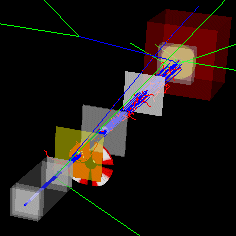
\includegraphics[height=1.75in,clip]{../figs/cco-beam}
  		%http://www.npl.co.uk/irmodelling/monte-carlo-workshop-and-mcneg-2007
	\end{center}
  	\end{figure}
  \end{column}
\end{columns}

\end{frame}


%%%%%%%%%%%%%%%%%%%%%%%%%%%%%%%%%%%%%%%%%%%%%%%%%%%%%%
%%%%%%%%%%%%%%%%%%%%%%%%%%%%%%%%%%%%%%%%%%%%%%%%%%%%%%
\begin{frame}{What is MC Radiation Transport?}

Simulate many independent particles in a system
\begin{itemize}
\item Treat each physical process as a
\textit{probabilistic process}
\pause
\item \textit{Randomly sample} each process using an
independent stream of random numbers
\pause
\item Follow each particle from birth until it no
longer matters
\pause
\item Accumulate the contributions of each
particle to find the statistically-expected
mean behavior and variance
\end{itemize}

\end{frame}


%%%%%%%%%%%%%%%%%%%%%%%%%%%%%%%%%%%%%%%%%%%%%%%%%%%%%%
%%%%%%%%%%%%%%%%%%%%%%%%%%%%%%%%%%%%%%%%%%%%%%%%%%%%%%
\begin{frame}{Mathematical Validity}

\begin{itemize}
\item Consider particles with a phase space
describing position, $\vec{r}$, and velocity, $\vec{v}$
\vspace*{0.5 em}
\item A neutral particle can be transmitted
from one position to another at a
constant velocity
\[T(\vec{r}\:' \rightarrow \vec{r}, \vec{v})\]
\pause
\item A particle can undergo a collision at a
single position that changes its velocity
\[C(\vec{r}, \vec{v}\:' \rightarrow \vec{v})\]
\end{itemize}

\end{frame}


%%%%%%%%%%%%%%%%%%%%%%%%%%%%%%%%%%%%%%%%%%%%%%%%%%%%%%
%%%%%%%%%%%%%%%%%%%%%%%%%%%%%%%%%%%%%%%%%%%%%%%%%%%%%%
\begin{frame}{Contributions After 0 Collisions}

\begin{itemize}
\item Consider a particle born from a source
described by 
\[Q(\vec{r}\:', \vec{v}\:')\]
\item This particle will contribute to the flux at $(\vec{r}, \vec{v})$ before any collisions
\end{itemize}

\[\psi_0(\vec{r}, \vec{v}) = \int_{\vec{r}\:'} Q(\vec{r}\:', \vec{v}\:')T(\vec{r}\:' \rightarrow \vec{r}, \vec{v}) d\vec{r}\:'\]

\end{frame}


%%%%%%%%%%%%%%%%%%%%%%%%%%%%%%%%%%%%%%%%%%%%%%%%%%%%%%
%%%%%%%%%%%%%%%%%%%%%%%%%%%%%%%%%%%%%%%%%%%%%%%%%%%%%%
\begin{frame}{Contributions After 1 Collision}

\begin{itemize}
\item The uncollided particles, $\psi_0(\vec{r}\:', \vec{v}\:')$, could undergo 1 \textcolor{cardinal}{collision} and then be \alert{transmitted} to the point $(\vec{r}, \vec{v})$
\end{itemize}

\[\psi_1(\vec{r}, \vec{v}) = \underbrace{\int_{\vec{r}\:'} \biggl[ \underbrace{\int_{\vec{v}\:'} \psi_0(\vec{r}\:', \vec{v}\:') C(\vec{r}\:', \vec{v}\:' \rightarrow \vec{v})  d\vec{v}\:'}_{\textcolor{cardinal}{collision}}\biggr] T(\vec{r}\:' \rightarrow \vec{r}, \vec{v}) d\vec{r}\:'}_{\alert{transmission}}\]

\end{frame}


%%%%%%%%%%%%%%%%%%%%%%%%%%%%%%%%%%%%%%%%%%%%%%%%%%%%%%
%%%%%%%%%%%%%%%%%%%%%%%%%%%%%%%%%%%%%%%%%%%%%%%%%%%%%%
\begin{frame}{Contributions After $k$ Collisions}

\begin{itemize}
\item Particles that have undergone $k$ collisions, $\psi_k(\vec{r}\:', \vec{v}\:')$, could undergo another \textcolor{cardinal}{collision} and then be \alert{transmitted} to the point $(\vec{r}, \vec{v})$ 
\end{itemize}

\[\psi_{k+1}(\vec{r}, \vec{v}) = \underbrace{\int_{\vec{r}\:'} \biggl[ \underbrace{\int_{\vec{v}\:'} \psi_k(\vec{r}\:', \vec{v}\:') C(\vec{r}\:', \vec{v}\:' \rightarrow \vec{v})  d\vec{v}\:'}_{\textcolor{cardinal}{collision}}\biggr] T(\vec{r}\:' \rightarrow \vec{r}, \vec{v}) d\vec{r}\:'}_{\alert{transmission}}\]

\end{frame}



%%%%%%%%%%%%%%%%%%%%%%%%%%%%%%%%%%%%%%%%%%%%%%%%%%%%%%
%%%%%%%%%%%%%%%%%%%%%%%%%%%%%%%%%%%%%%%%%%%%%%%%%%%%%%
\begin{frame}{Combine Collision and Transmission Kernels}

\begin{align*}
\vec{p} &= (\vec{r}, \vec{v}) \quad \text{and}\\
%
R(\vec{p}\:'\rightarrow\vec{p}) &\equiv C(\vec{r}\:', \vec{v}\:' \rightarrow \vec{v}) T(\vec{r}\:' \rightarrow \vec{r}, \vec{v}) \\
&\\
%
\psi_{k+1}(\vec{r}, \vec{v}) = \int_{\vec{p}_k} \psi_k(\vec{p}_k) &R(\vec{p}_k \rightarrow \vec{p}_{k+1}) d\vec{p}_k \\
%
&\\
\psi_{k+1}(\vec{r}, \vec{v}) = \int_{\vec{p}_k} \biggl[ \int_{\vec{p}_{k-1}}  &\psi_{k-1}(\vec{p}_{k-1}) R(\vec{p}_{k-1} \rightarrow \vec{p}_{k}) d\vec{p}_{k-1} \biggr] R(\vec{p}_k \rightarrow \vec{p}_{k+1}) d\vec{p}_k \\
&\text{\dots and so on \dots}
&\\
\psi_{k+1}(\vec{r}, \vec{v}) = \int_{\vec{p}_k} &\int_{\vec{p}_{k-1}} \cdots \int_{\vec{p}_0} \psi_{0}(\vec{p}_{0}) R(\vec{p}_{0} \rightarrow \vec{p}_{1}) d\vec{p}_{0} \cdots \\
&\psi_{k-1}(\vec{p}_{k-1}) R(\vec{p}_{k-1} \rightarrow \vec{p}_{k}) d\vec{p}_{k-1} R(\vec{p}_k \rightarrow \vec{p}_{k+1}) d\vec{p}_k \\
\end{align*}

\end{frame}


%%%%%%%%%%%%%%%%%%%%%%%%%%%%%%%%%%%%%%%%%%%%%%%%%%%%%%
%%%%%%%%%%%%%%%%%%%%%%%%%%%%%%%%%%%%%%%%%%%%%%%%%%%%%%
\begin{frame}{Sum Over All Collisions}

\[\psi(\vec{p}) = \sum_{k=0}^{\infty} \psi_k(\vec{p})\]

\vspace*{1 em}
Arriving at the \textit{integral form} of the transport equation

\[\psi(\vec{r}, \vec{v}) = \int_{\vec{r}\:'} \biggl[ \int_{\vec{v}\:'} \psi(\vec{r}\:', \vec{v}\:') C(\vec{r}\:', \vec{v}\:' \rightarrow \vec{v})  d\vec{v}\:'\biggr] T(\vec{r}\:' \rightarrow \vec{r}, \vec{v}) d\vec{r}\:'\]

\end{frame}


%%%%%%%%%%%%%%%%%%%%%%%%%%%%%%%%%%%%%%%%%%%%%%%%%%%%%%
%%%%%%%%%%%%%%%%%%%%%%%%%%%%%%%%%%%%%%%%%%%%%%%%%%%%%%
\begin{frame}{Mathematical Validity}

\begin{align*}
\Psi_{k}(\vec{p}) = \int\int &\cdots \int \Psi_{0}(\vec{p}_{0}) R(\vec{p}_{0} \rightarrow \vec{p}_{1})R(\vec{p}_{1} \rightarrow \vec{p}_{2}) \\&\cdots R(\vec{p}_{k-1} \rightarrow \vec{p}_{k}) d\vec{p}_{0} d\vec{p}_{1} \cdots d\vec{p}_{k-1}
\end{align*}

\begin{itemize}
\item Integration over many variables
\hspace*{0.5 em}
\item Generate a ``history"\\
(sequence of states $\vec{p}_0, \vec{p}_1 , \dots, \vec{p}_k$)
\begin{itemize}
 \item Randomly sample from source: $\Psi_0 (\vec{p}_0)$
 \item Randomly sample for each of $k$ transitions: $R(\vec{p}_{k-1} \rightarrow \vec{p}_{k})$
\end{itemize}
\pause
\item Average for result $A$ by averaging of $M$ histories
\end{itemize}

\[\left\langle A \right\rangle = \int A(\vec{p})\Psi(\vec{p}) d\vec{p} 
= \frac{1}{M} \sum_{m=1}^M \biggl[ \sum_{k=1}^{\infty} A(\vec{p}_{k,m}) \Psi(\vec{p}_{k,m}) \biggr] \]

\end{frame}


%%%%%%%%%%%%%%%%%%%%%%%%%%%%%%%%%%%%%%%%%%%%%%%%%%%%%%
%%%%%%%%%%%%%%%%%%%%%%%%%%%%%%%%%%%%%%%%%%%%%%%%%%%%%%
\begin{frame}{Can Model Very Complex Things}

  	\begin{figure}
  	\begin{center}
  		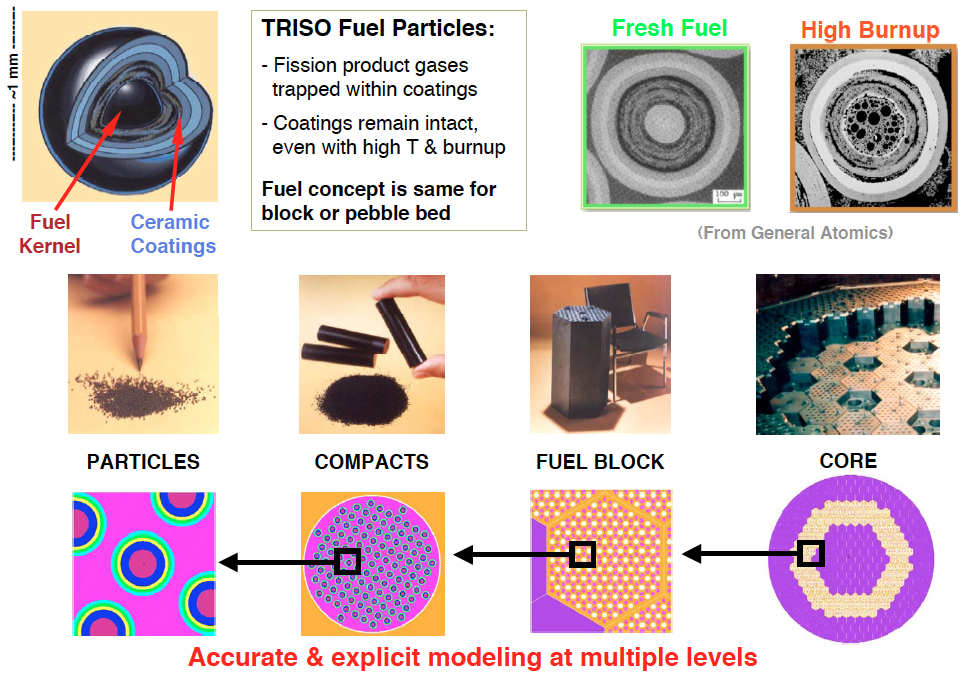
\includegraphics[height=3in,clip]{../figs/pbmr}
	\end{center}
  	\end{figure}

\end{frame}

\end{document}
